%15 min preso!
\documentclass[xcolor=table,aspectratio=169]{beamer}
\usepackage{beamerthemesplit}
\usepackage{wrapfig}
\usetheme{SPbGU}
\usepackage{pdfpages}
\usepackage{amsmath}
\usepackage{cmap}
\usepackage[T2A]{fontenc}
\usepackage[utf8]{inputenc}
\usepackage[english]{babel}
\usepackage{indentfirst}
\usepackage{amsmath}
\usepackage{tikz}
\usepackage{multirow}
\usepackage[noend]{algpseudocode}
\usepackage{algorithm}
\usepackage{algorithmicx}
\usepackage{fancyvrb}
\usepackage{hyperref} 
\usetikzlibrary{calc}
\usetikzlibrary{shapes, backgrounds}
\usetikzlibrary{arrows,automata}
\usetikzlibrary{positioning}
\usetikzlibrary{fit}
\usetikzlibrary{shapes.callouts}
\usetikzlibrary{shapes.misc}
\usepackage{xparse}
\usepackage{fontawesome}

\usepackage{etoolbox,refcount}
\usepackage{multicol}

\usepackage{tabularx}
\newcolumntype{Y}{>{\raggedleft\arraybackslash}X}

\renewcommand{\thealgorithm}{}

\newtheorem{mytheorem}{Theorem}
\renewcommand{\thealgorithm}{}

\newcommand{\tikzmark}[1]{\tikz[overlay,remember picture] \node (#1) {};}
\def\Put(#1,#2)#3{\leavevmode\makebox(0,0){\put(#1,#2){#3}}}

\newcommand{\ltz}{$< 1$}

\tikzset{
    state/.style={
           rectangle,
           rounded corners,
           draw=black, very thick,
           minimum height=2em,
           inner sep=2pt,
           text centered,
           },
}

\tikzset{
    invisible/.style={opacity=0,text opacity=0},
    visible on/.style={alt=#1{}{invisible}},
    alt/.code args={<#1>#2#3}{%
      \alt<#1>{\pgfkeysalso{#2}}{\pgfkeysalso{#3}} % \pgfkeysalso doesn't change the path
    },
}

\tikzset{cross/.style={cross out, draw=black, minimum size=2*(#1-\pgflinewidth), inner sep=0pt, outer sep=0pt, ultra thick},
%default radius will be 1pt. 
cross/.default={1pt}}

\NewDocumentCommand{\mycallout}{r<> O{opacity=0.8,text opacity=1} m m m}{%
\tikz[remember picture, overlay]\node[align=center, fill=cyan!20, text width=#5cm,
#2,visible on=<#1>, rounded corners,
draw,rectangle callout,anchor=pointer,callout relative pointer={(290:0.5cm)}]
at (#3) {#4};
}

\NewDocumentCommand{\mycalloutR}{r<> O{opacity=0.8,text opacity=1} m m m}{%
\tikz[remember picture, overlay]\node[align=center, fill=cyan!20, text width=#5cm,
#2,visible on=<#1>, rounded corners,
draw,rectangle callout,anchor=pointer,callout relative pointer={(30:0.8cm)}]
at (#3) {#4};
}


%callout relative pointer={(230:0.5cm)}]

\newcounter{countitems}
\newcounter{nextitemizecount}
\newcommand{\setupcountitems}{%
  \stepcounter{nextitemizecount}%
  \setcounter{countitems}{0}%
  \preto\item{\stepcounter{countitems}}%
}
\makeatletter
\newcommand{\computecountitems}{%
  \edef\@currentlabel{\number\c@countitems}%
  \label{countitems@\number\numexpr\value{nextitemizecount}-1\relax}%
}
\newcommand{\nextitemizecount}{%
  \getrefnumber{countitems@\number\c@nextitemizecount}%
}
\newcommand{\previtemizecount}{%
  \getrefnumber{countitems@\number\numexpr\value{nextitemizecount}-1\relax}%
}
\makeatother    
\newenvironment{AutoMultiColItemize}{%
\ifnumcomp{\nextitemizecount}{>}{3}{\begin{multicols}{2}}{}%
\setupcountitems\begin{itemize}}%
{\end{itemize}%
\unskip\computecountitems\ifnumcomp{\previtemizecount}{>}{3}{\end{multicols}}{}}


\beamertemplatenavigationsymbolsempty

\title[Research Group Report]{Summer Report}
\institute[SPbSU]{
Saint Petersburg State University
}

% То, что в квадратных скобках, отображается в левом нижнем углу.
\author[Semyon Grigorev]{Semyon Grigorev}

\date{August 31, 2023}



\begin{document}
{
\begin{frame}[fragile]
  \begin{table}
  \centering
  %
\includegraphics[height=1.5cm]{pictures/SPbGU_Logo.png}
  \begin{tabularx}{\linewidth}{XcX}
    
\includegraphics[height=0.9cm]{pictures/hu_logo.jpeg} \hfill
    & 
    & \hfill 
\includegraphics[height=1.6cm]{pictures/SPbGU_Logo.png}
  \end{tabularx}
  \end{table}
  \titlepage
\end{frame}
}

%\begin{frame}[fragile]
%  \frametitle{Research Landscape}  
%  \begin{center}
%    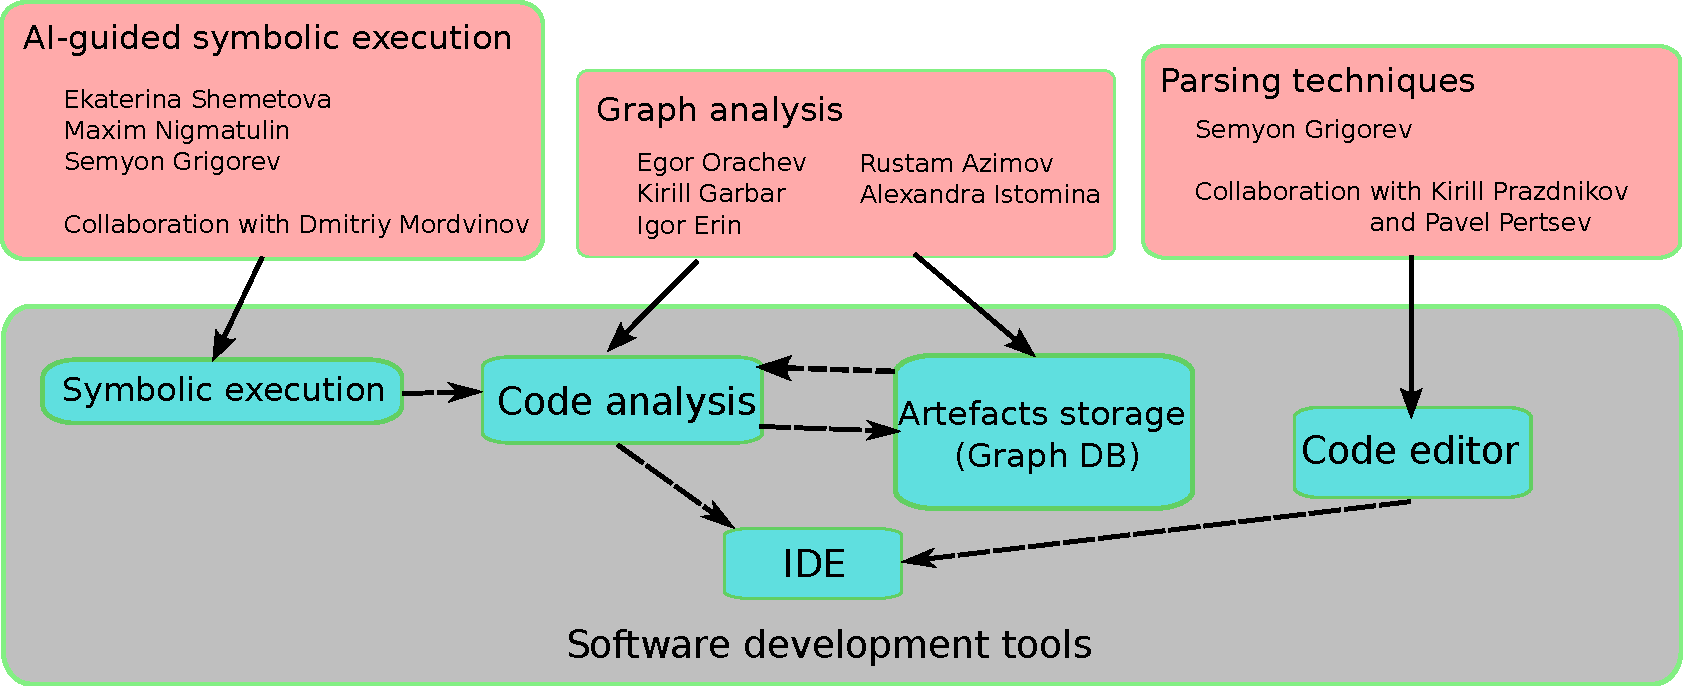
\includegraphics[width=\textwidth]{pictures/landscape.pdf}
%  \end{center} 
%\end{frame}


\begin{frame}[fragile]
  \frametitle{$\mathcal{AI}$-Guided Symbolic Execution}
  \begin{itemize}
  \item[\faGroup] Maxim Nigmatulin, Ekaterina Shemetova, Anna Chistyakova
  \end{itemize}
  \vspace{0.5cm}
  \begin{minipage}{0.49\textwidth}
  \begin{itemize}
    \item[\faCheck] Infrastructure for training
    \item[\faCheck] Basic dataset
    \item[\faCheck] Basic integration with USVM
    \item[\faCheck] Basic evaluation
  \end{itemize}  
  \end{minipage}
  \begin{minipage}{0.49\textwidth}
  \begin{itemize}
    \item[\faGears] Full integration with USVM
    \item[\faGears] Dataset extension
    \item[\faGears] GNN improvement and training 
    \item[\faGears] Performance tuning
  \end{itemize}  
  \end{minipage}


  \begin{center}  
    \begin{tabular}{l |c c |c c |c c |c c }
      \hline 
      \multirow{2}{*}{Searcher} & \multicolumn{2}{c|}{Coverage} & \multicolumn{2}{c|}{Steps} & \multicolumn{2}{c|}{Tests} & \multicolumn{2}{c}{Errors} \\
                                & Mean & Median                & Mean & Median             &  Mean & Median            & Mean & Median                 \\
      \hline 
      $\mathcal{AI}$            &  100 &    100                &  300 & 300                &  1    &  1                &  1   &  1                     \\
      $\mathcal{BFS}$           &      &                       &      &                    &       &                   &      &                        \\
      $\mathcal{!!!}$           &      &                       &      &                    &       &                   &      &                        \\
      $\mathcal{!!!}$           &      &                       &      &                    &       &                   &      &                        \\
      \hline 
    \end{tabular}
  \end{center}
  
\end{frame}


\begin{frame}[fragile]
  \frametitle{Other Projects}
  
  \begin{itemize}
    \item[\faCheck] Datalog-based static code analysis (Rustam Azimov)
    \begin{itemize}
      \item[\faFrownO] Pure Datalog is not flexible enough
      \item[\faGears] Switched to IFDS-based analysis
    \end{itemize}
    \item[\faGears] SAT on GPGPU (Egor Orachev)
    \begin{itemize}
      \item[\faCheck] First prototype
      \item[\faGears] GNN + SAT + GPGPU: can it be used in $\mathcal{AI}+SE$ pipeline 
    \end{itemize}
    \item[\faGears] High-performance graph analysis (Egor Orachev, Igor Erin, Artemii Patov)
    \begin{itemize}
      \item[\faCheck] Paper
      \item[\faGears] Core refactoring
      \item[\faGears] Package publishing
    \end{itemize}
  \end{itemize}
\end{frame}

\end{document}
